%!TEX program = xelatex
%!TEX TS-program = xelatex
%!TEX encoding = UTF-8 Unicode

\documentclass[12pt, a4paper]{article} % A4 纸,字体大小为 12pt 的 article 类文档
\usepackage{CJKutf8} % 中文支持
\usepackage{graphicx} % 插入图片
\usepackage{subfigure} % 插入多图时用子图显示的宏包
\usepackage{listings} % 支持代码显示
\usepackage[colorlinks,linkcolor=blue]{hyperref} % 超链接
\usepackage{ulem} % 删除线
\usepackage{xcolor} % 定制颜色
\usepackage{caption2} % 浮动图形和表格标题样式
\usepackage{amssymb} % 数学符号
\usepackage{indentfirst} % 中文段落首行缩进
\usepackage{tikz} % 画图
\usepackage{pgfplots} % 画图
\usepackage{amsmath} % 处理数学公式
\usepackage{mathtools} % 处理数学公式
\setlength{\parskip}{0.5em} % 段落间距
\renewcommand{\figurename}{图} % 将图表的标题设置为中文“图”
\usetikzlibrary{tikzmark,calc,decorations.pathreplacing} % tikzmark 用于标记位置,calc 用于计算,decorations.pathreplacing 用于画大括号


\title{第二十二·演化博弈·有限理性与动态均衡}
\author{hoochanlon}
\date{\today}

\begin{document}
	\begin{CJK*}{UTF8}{gbsn}
		\maketitle
        \clearpage
        \section{演化博弈理论}
        \subsection{演化博弈理论的起源}
        演化博弈理论也称为进化博弈论。根据达尔文的理论,自然选择发生在个体层面,所以自利行为会被奖励,而利他的行为并不会得到奖励。适者生存逼迫动物们必须是恶的,
        所有的善都会被淘汰。这个问题可以用演化博弈论来解释,在演化博弈中,参与者选择的策略可以是理性的,也可以是非理性的,可以是恶的,也可以是善的。
        然后参与者彼此博弈,博弈出来的结果会去检验这个策略,是成功的,还是失败的。\textbf{之所以称之为演化,是因为通过一代又一代的演化来检验不同策略,
        在环境中的生存和复制能力}。

        \subsection{演化博弈基本概念}
        演化博弈论是一种把博弈论和动态演化过程结合起来的理论,传统的博弈论中有许多均衡的概念,比如说“纳什均衡”、“子博弈完美纳什均衡”、“贝叶斯纳什均衡”等。
        对均衡的研究一直是博弈论研究的核心内容,演化博弈论的核心概念是 \textbf{演化稳定策略(ESS)}。其基本思想如下:

        \begin{itemize}
            \item[] 如果一个初始群体的某种行为模式能够消除任何小的突变群体,那么这种行为模式一定能够获得比突变群体更高的收益。随着时间的演化,
                    突变者群体最后会从初始群体中消失。由此初始群体所选择的策略,就是演化稳定策略。系统选择演化稳定策略时所处的状态是演化稳定状态,
                    由此建立的均衡,就是演化稳定均衡。
        \end{itemize}

        之前建立的博弈分析都是建立在参与人是理性人的基础上,而演化稳定策略不需要建立在完全理性的基础上,只需要建立在有限理性基础上。因此演化博弈均衡
        可以看做是纳什均衡的一种精炼。ESS一定是纳什均衡,但并非所有的纳什均衡都是ESS。对演化过程的分析,可以很好的帮助我们选择某种特定的纳什均衡。
        在ESS的基础上,研究者进一步提出了叫模仿者动态的概念。

        \clearpage
        \section{模仿者动态与分析框架}
        \subsection{模仿者动态}
        当一种策略得到的适应值高于群体的平均适应值,群体中采用这种策略的成员就会增加,反之则会减少。模拟者动态能够较好的描绘出有限理性个体的群体行为变化趋势,
        由此得出的结论能够比较准确地预测个体的群体行为。模仿者动态与演化稳定策略一起构成演化博弈理论最核心的一对基本概念,它们分别表征演化博弈的稳定状态
        和向这种稳定状态的动态收敛过程。

        \subsection{分析框架}
        演化博弈源于对生物进化的研究,那么生物进化论有三个基本基础性假设:异质性、适应性、选择。基因的多样性导致群种的异质性,物种对环境的适应性,
        决定其基因是否能被遗传。物竞天择是指生存的动态选择。这个过程改变物种之间的生存状态和相互关系。随着时间的推移,偶然因素会带来新的基因变异,
        如果该变异不能适应环境,则最终将消亡。如果该变异能够实现一种更强的适应性,就会成功的侵入这个群体,并成为种群的一个重要组成部分。
        当种群不能被任何变异成功侵入时,生物学家就将该种群结构及其当前表现型是进化稳定的。\par

        \textbf{演化稳定状态可能只有一个策略,也可能包含多个具有同样适应性的行为方式,前者叫单元均衡,后者是多元均衡}。演化博弈的多元均衡不需要参与者采用混合策略,
        \textbf{每个参与者完全可以选择纯策略,但种群中会因不同参与者选择了不同的纯策略,而呈现出一种混合式的多元均衡}。

        \subsubsection{演化博弈模型特征}
        \begin{enumerate}
            \item 以参与人群体为研究对象,分析动态的演化过程,解释群体为何达到以及如何达到这一状态。
            \item 群体的演化既有选择过程,也有突变过程。
            \item 经群体选择下来的行为具有一定惯性。(从众)
        \end{enumerate}

        不难看出,在之前的博弈分析中,如果纳什均衡存在,那么博弈双方就直接达到了纳什均衡。纳什均衡往往不依赖于初始状态,不需要任何的动态调整过程。
        而在演化博弈中,这个ESS它均衡的达成,往往需要多次博弈后才能达到,需要一个动态的调整过程,因此演化博弈的均衡达成是依赖初始状态的,
        有着明显的路径依赖过程。

        \clearpage
        \section{演化博弈模型分析}
        \subsection{鹰鸽博弈的演化稳定策略(ESS)}
        可以把鹰鸽博弈理解为一个群体内部参与者为争夺总量是2A的资源的一个博弈。老鹰代表强硬,类似懦夫博弈中的“进”,鸽子代表温和类似懦夫博弈中的“退”。
        如果双方都选鸽子,那么就平分2A;如果一方老鹰,一方鸽子;那么老鹰独占2A,如果双方都老鹰,各自A-C(C代表争斗的损耗)。

        \begin{figure}[htbp]
            \centering
            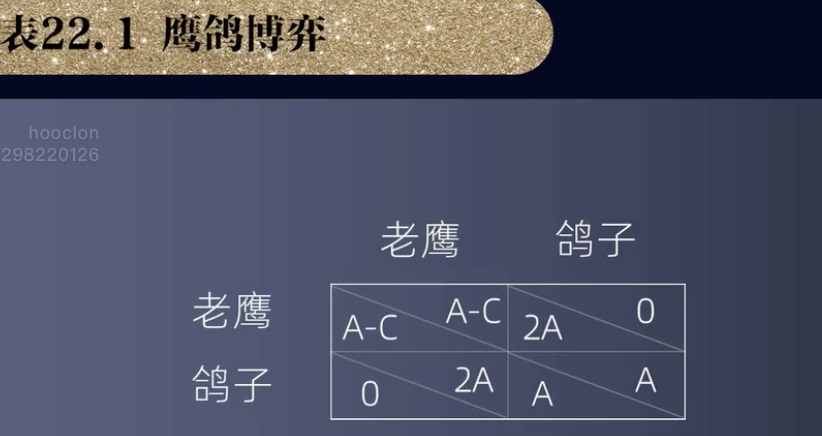
\includegraphics[width=1\textwidth]{./figures/catch2023-08-05-16.34.54.png}
            \caption{鹰鸽博弈的收益矩阵}
        \end{figure}

        该模型的纳什均衡分两种情况进行分析,第一种情况是 $A > C$ 选老鹰是占优策略,双方老鹰为纳什均衡解。$A < C$ 该博弈存在两个纯策略
        (老鹰,鸽子;鸽子,老鹰)的纳什均衡,和混合策略的纳什均衡。

        \subsection{鹰鸽博弈混合策略纳什均衡求解}
        假设:任何一方选择老鹰的概率为 $\alpha$,选择鸽子的概率为 $1- \alpha$。

        \begin{itemize}
            \item[] $\alpha(A-C)+2A=A(1-\alpha)$
            \item[] $\alpha=A/C$
        \end{itemize}

        当任何一方选择老鹰是 $\frac{A}{C}$ 那么任何一方选择老鹰或鸽子的期望收益是相等的,那么由此构成混合策略纳什均衡。接下来我们以演化博弈的角度来分析鹰鸽博弈。
        在A小于C的情况下面,如果群体中所有的参与者都是老鹰组成,那么每次的博弈结果就是$A-C<0$。更大的收益代表更强的适应性,那么当损益小于0的时候,就意味着对环境的适应性
        是不断下降的。那么在全体老鹰的群体中,一旦出现基因变异了,变异成鸽子的个体损益是0,那么这个损益为0的,反而在群体中会有更大适应性,并在后续的遗传中获得优势。
        由此就出现老鹰比例不断下降,鸽子比例不断上升的演化过程。反之同理。\par

        老鹰占比为 $\frac{A}{C}$ 的时候就是ESS,如果老鹰比例大于 $\frac{A}{C}$ 老鹰适应性下降,鸽子适应性上升。从演化的视角看来,鹰鸽博弈其实是多元均衡。

        \subsection{语言博弈的演化稳定策略(ESS)}

        常规形态:都说英语的收益是2,都说汉语的收益是1;在这个模型中有两个纯策略纳什均衡,以及一个混合策略纳什均衡,即:1/3英语,2/3汉语。如果对方有1/3的可能性说英语,
        2/3的可能性会说汉语,那么对于你来说学习说英语的收益是等同于汉语的期望收益。

        \begin{figure}[htbp]
            \centering
            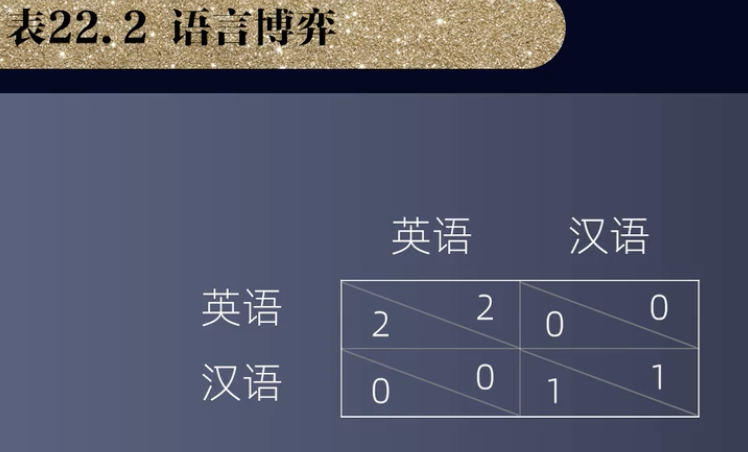
\includegraphics[width=1\textwidth]{./figures/catch2023-08-05-17.19.58.png}
            \caption{语言博弈的收益矩阵}
        \end{figure}

        演化博弈分析:如果群体全部都说英语,那么这个时候变异成说汉语的个体,他的适应性下降,反之亦然。因此该博弈的ESS要么都说英语,要么都说汉语。
        至于前面所提的“1/3英语,2/3汉语”,它不是ESS,从众才是每个参与者的ESS。

        \subsection{囚犯困境的ESS}
        \subsubsection{囚犯困境单次博弈}
        \begin{figure}[htbp]
            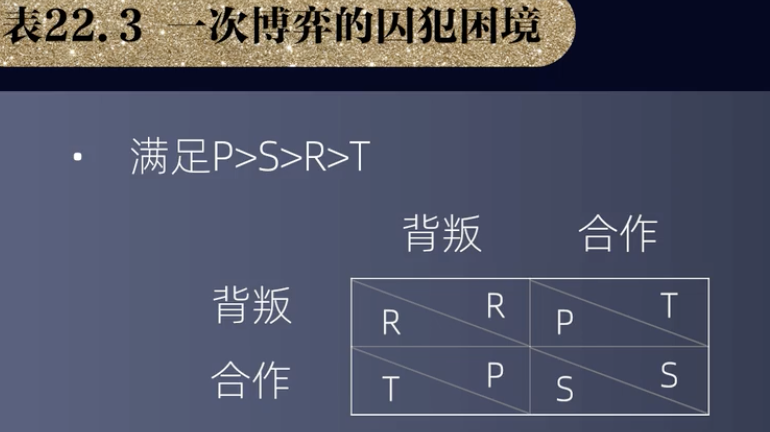
\includegraphics[width=0.7\textwidth]{./figures/catch2023-08-05-17.34.34.png}
        \end{figure}

        \begin{figure}[htbp]
            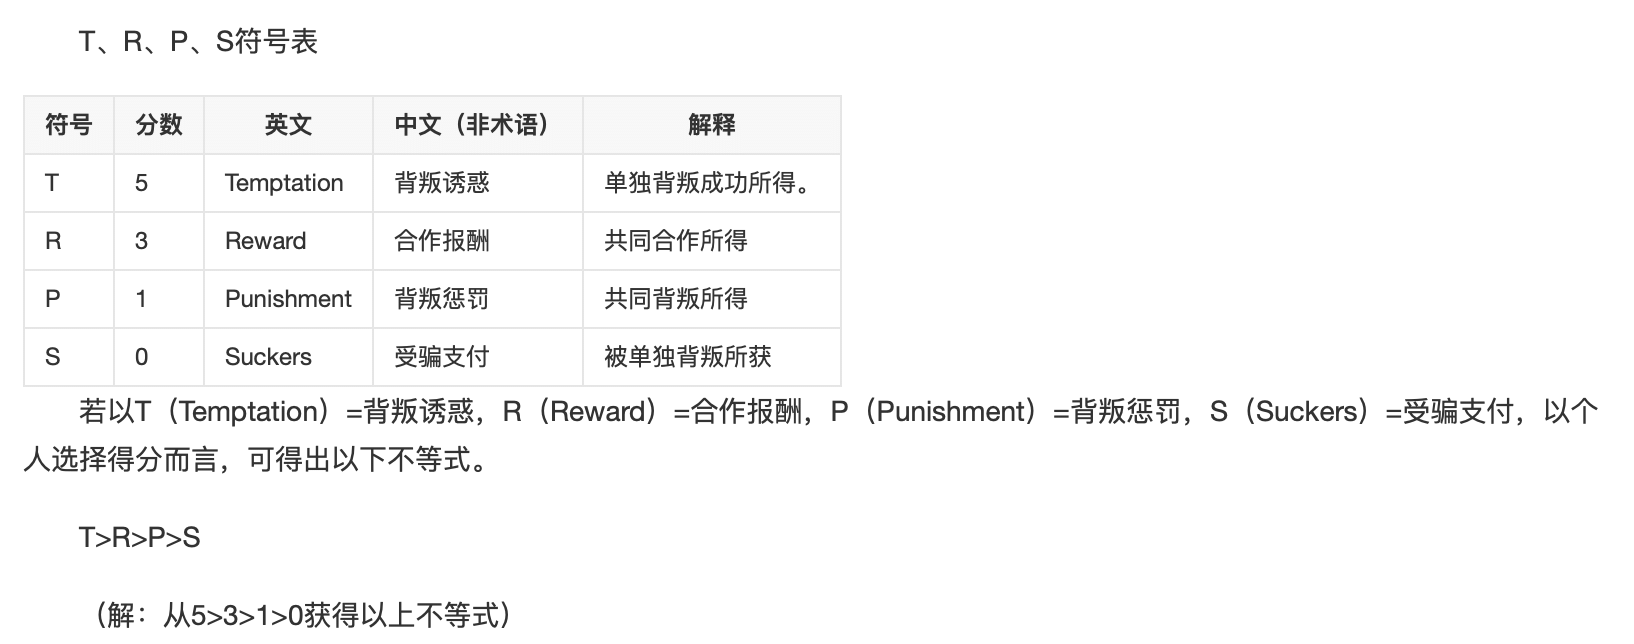
\includegraphics[width=1\textwidth]{./figures/catch2023-08-05-17.47.51.png}
        \end{figure}

        设遭遇对手选择背叛的概率为 $\alpha$ 合作的概率为 $1-\alpha$。选择背叛的期望收益为 $\alpha R+(1-\alpha)P$,选择合作的期望收益为
         $\alpha T+(1-\alpha)S$。所以,背叛的期望收益严格大于合作期望收益。因此,一个群体无论一开始合作型的占比是多少,其演化的必然结果是
         所有参与者都成为背叛型,合作的基因变异无法入侵该群体。总之,一个博弈里有严格的占优策略,那么该策略必然是ESS \par

        \subsubsection{囚犯困境重复二次博弈}
        重复博弈的六种策略:\par
        \begin{enumerate}
            \item 一直合作。
            \item 第一次背叛,对方背叛则背叛,对方合作则合作。
            \item 第一次背叛,对方背叛则合作,对方合作则背叛。
            \item 第一次合作,对方背叛则合作,对方合作则背叛。
            \item 第一次合作,对方背叛则背叛,对方合作则合作。
            \item 两次都背叛。
        \end{enumerate}

        \begin{figure}[htbp]
            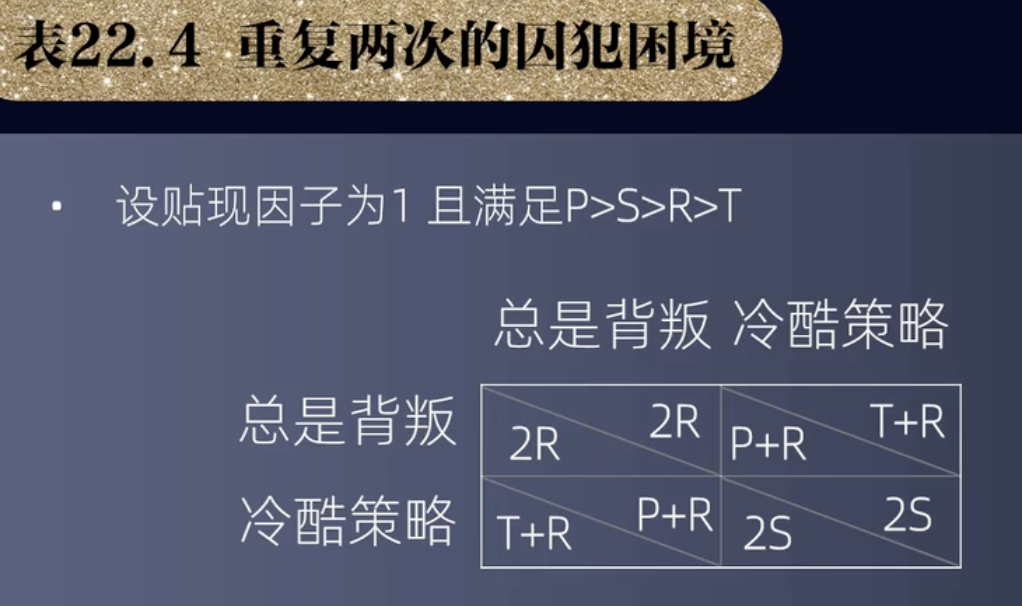
\includegraphics[width=1\textwidth]{./figures/catch2023-08-05-18.11.12.png}
        \end{figure}

        设总是背叛类型的占比为 $\alpha$ 冷酷策略的占比则为$1- \alpha$。那么,总是背叛的期望收益为 $\alpha R+(1-\alpha)(P+R)$
        ,冷酷策略的期望收益为$\alpha (T+R) + 2(1-\alpha)S$ 。由此 $ 2 \alpha R+(1-\alpha)(P+R)>\alpha(T+R)+2(1-\alpha)S$ 。

        \subsubsection{囚犯困境重复N次博弈}

        设总是背叛的类型占比为$\alpha$,冷酷策略的占比则为$1-\alpha$。那么,总是背叛的期望收益为$\alpha N+(1-\alpha)(N+4))$
        冷酷策略的期望收益为$\alpha (N-1) + 3N(1-\alpha)$;$\alpha=1-1/(2N-3)$

        \begin{figure}[htbp]
            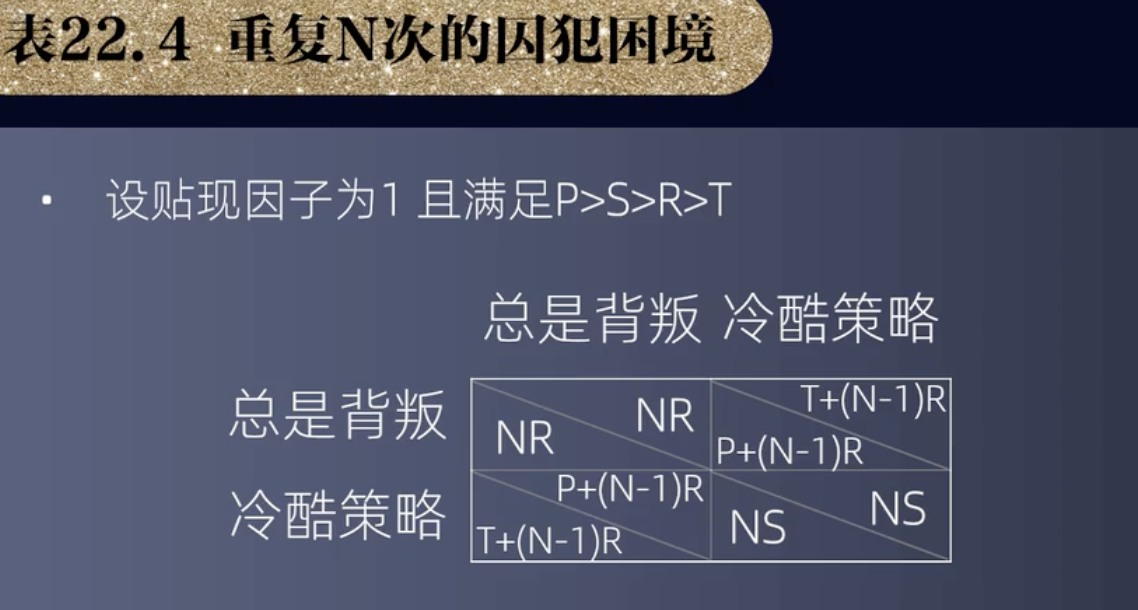
\includegraphics[width=1\textwidth]{./figures/catch2023-08-05-18.37.37.png}
            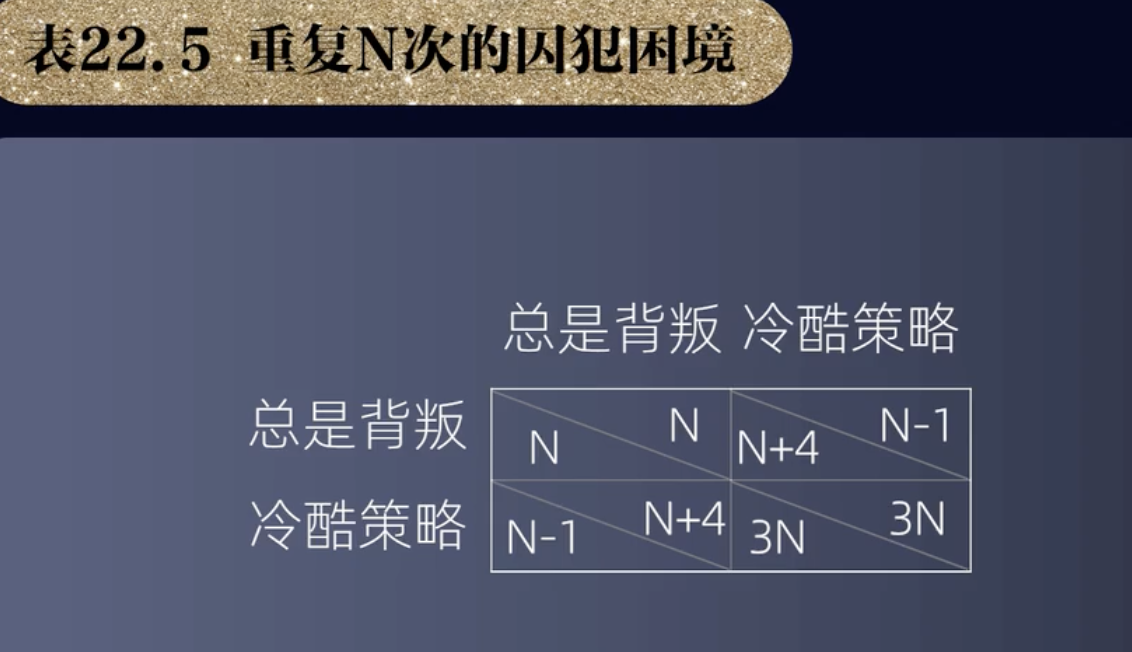
\includegraphics[width=1\textwidth]{./figures/catch2023-08-05-18.38.40.png}
        \end{figure}

        当群体中总是背叛型的占比为$1-1/(2N-3)$,或者冷酷策略的占比为$1/(2N-3)$时,每个参与者的期望收益其实是相等的。如果N=3,当群体中总是背叛
        的占比超过2/3的时候,总是背叛的期望收益是大于冷酷策略的,总是背叛是ESS。当群体中总是背叛占比小于2/3的时候,总是冷酷策略是ESS。总是背叛,
        还是总是冷酷策略的演化结果取决于初始条件。当N无限大,群体交往比例越高,合作的可能性越大。\par

        \textbf{总结:}在重复博弈中,如果博弈次数足够多,那么合作是ESS。如果博弈次数有限,那么总是背叛是ESS。如果博弈次数有限,那么总是背叛是ESS。

        \subsection{损人害己}
        损人害己看上去好像是非理性的行为,好像不符合博弈论的基本假设,但又是现实生活中我们司空见惯的事情。

        \begin{figure}[htbp]
            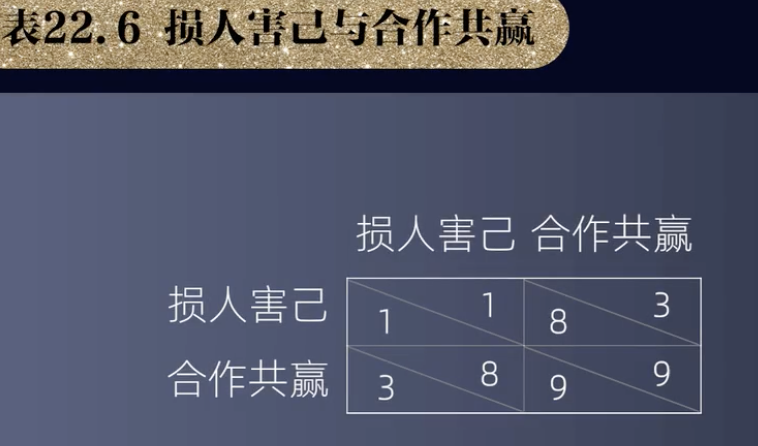
\includegraphics[width=1\textwidth]{./figures/catch2023-08-05-19.07.45.png}
        \end{figure}

        从演化的博弈视角来看,合作共赢并不是ESS,参与者的适应度是有其收益的相对值决定的,那个损人害己的参与者,由此反而获得了更大适应度,这也就解释了
        哪怕那种所谓的叫自伤八百杀敌一千的说法,其结果大大降低了群体的适应性,这相当于是演化博弈中的囚犯困境。

        \subsection{三方博弈的ESS}
        三方博弈是指三个参与者的博弈,每个参与者有三种策略:

        \begin{figure}[htbp]
            \subfigure[三方一次性博弈]{
                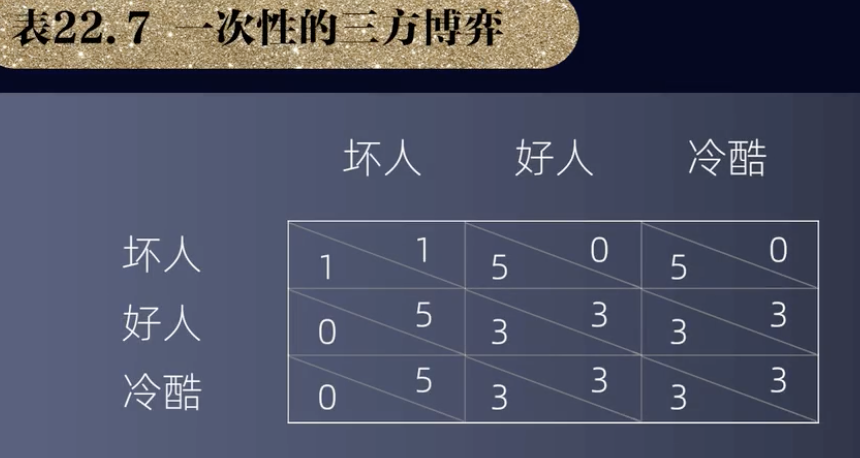
\includegraphics[width=0.5\textwidth]{./figures/catch2023-08-05-19.50.45.png}
            }
            \subfigure[三方的重复博弈]{
                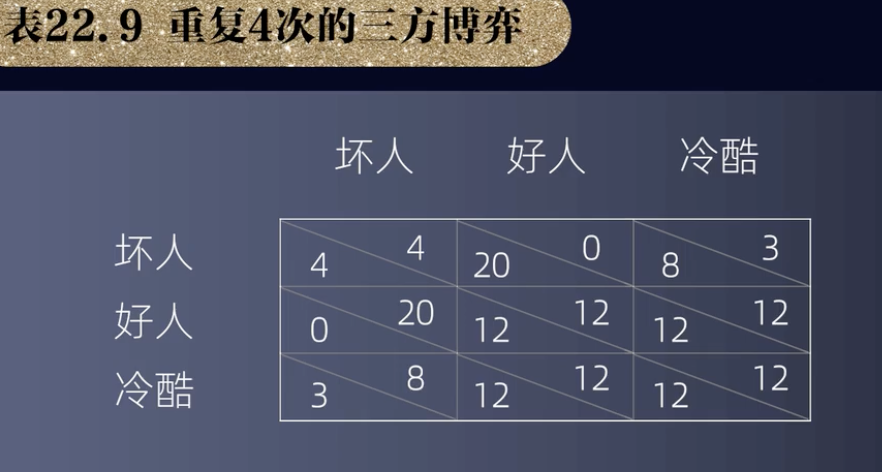
\includegraphics[width=0.5\textwidth]{./figures/catch2023-08-05-19.53.50.png}
            }
        \end{figure}

         \subsubsection{总结}
         \textbf{\textcolor{cyan}{如果群体中没有冷酷类型,坏人是占优策略,并成为ESS。有了冷酷类型后,三种策略没有一种策略是占优策略,不存在占优策略纳什均衡。
         当引入复制者动态后,该博弈不存在ESS。当坏人的比例足够大时,所有人都变坏成为演化均衡。}} \par

         \textbf{\textcolor{red}{好人之所以能够生存,是因为有大量的冷酷者帮助惩罚了那个坏人,降低了坏人的适应度。
         好人与冷酷者只有在面对坏人时才会显示差异特征,而在合作关系中难以被区分。这里存在的风险就是,因为两者具有相同适应度,当冷酷者变异成好人,
         好人比例逐步上升,当好人上升到一定程度,坏人比例也会因此增加,获得更大的适应度,这个群体的合作规范就被瓦解了,群体进入坏人当道的均衡结果。}} \par

         \textbf{一个社会当丧失了对坏人的惩罚机制,就会很容易进入到叫黑暗森林,就是所有人对所有人战争的状态。}

















    \end{CJK*}
\end{document}
